\documentclass[12pt]{article}
\usepackage[hidelinks]{hyperref}
\newtheorem{theorem}{Theorem}
\usepackage{xcolor}
\usepackage{textcomp}
\usepackage[italian]{babel}
\usepackage{graphicx}
\usepackage{outlines}
\newcommand{\circumdelta}{%
  \leavevmode\vbox{
    \offinterlineskip
    \ialign{%
      \hfil##\hfil\cr
      \^{}\cr\noalign{\vskip-1ex}
      $\delta$\cr
    }
  }%
}

\begin{document}
\tableofcontents
\newpage

\section{Introduzione}
\subsection{Motivazione} 
Un linguaggio è uno strumento per descrivere come risolvere i problemi in maniera rigorosa, in modo tale che sia eseguibile da un calcolatore
Perché è utile studiare come creare un linguaggio di programmazione? 
\begin{itemize}
  \item non rimanere degli utilizzatori passivi
  \item capire il funzionamento dietro le quinte di un linguaggio
  \item domain-specific language (DSL): è un linguaggio pensato per uno specifico problema
  \item model drivern software development: modo complesso per dire UML e simili
  \item model checking
\end{itemize}


\subsection{Definizioni base} 
Un linguaggio è composto da:
\begin{itemize}
  \item lessico e sintassi
  \item compilatore: parser + generatore di codice oggetto
\end{itemize}
La generazione automatica di codice può essere dichiarativa lessico
(espressioni regolari o automa a stati finite) o sintassi(grammatiche o automa a pile).
Un automa a stati finiti consuma informazioni una alla volta, ne salva una quantità finita. Alcuni esempi di applicazione di automa a stati finiti: software di progettazione di circuiti, analizzatore lessicale, ricerca di parole sul web e protocolli di comunicazione.

\begin{figure}[h]
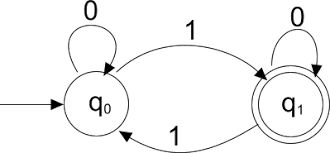
\includegraphics[scale = 0.3]{media/semplice_automa.png}
\centering
\caption{Semplice automa}
\end{figure}

\subsection{Contenuti del corso}
\begin{outline}
  \1 Linguaggi formali e Automi:
    \2 Automi a stati finiti, espressioni regolari, grammatiche libere, automi a pila, Macchine di Turing, calcolabilità
  \1 Compilatori:
    \2 Analisi lessicale, analisi sintattica, analisi semantica, generazione di codice
  \1 Logica di base:
    \2 Logica delle proposizioni e dei predicati
  \1 Modelli computazionali:
    \2 Specifica di sistemi tramite sistemi di transizione, logiche temporali per la specifica e verifica di proprietà dei sistemi (model checking), sistemi concorrenti (algebre di processi e reti di Petri)
\end{outline}

\subsection{Informazioni utili}
Parte integrante del corso:
\begin{outline}
  \1 Supporto alla parte teorica usando tool specifici.
  \2 JFLAP 7.1: http://www.jflap.org (automi/grammatiche)
  \2 Tina 3.7.5: http://projects.laas.fr/tina
  (model checking di sistemi di transizione e reti di Petri)
  \2 LTSA 3.0: http://www.doc.ic.ac.uk/ltsa
  (sistemi di transizione definiti tramite algebre di processi)
  \1 Nel resto del corso utilizzeremo un ambiente di sviluppo per
  generare parser/compilatori
  \2 IntelliJ esteso con plug-in ANTLRv4, ultima versione 1.20
  (generatore ANTLR: http://www.antlr.org/)
\end{outline}

\newpage
Libri di testo suggeriti:
\begin{outline}
 \1 J. E. Hopcroft, R. Motwani e J. D. Ullman:
Automi, linguaggi e calcolabilita’,
Addison-Wesley, Terza Edizione, 2009. Cap. 1–9
\1 A. V. Aho, M. S. Lam, R. Sethi e J. D. Ullman:
Compilatori: principi tecniche e strumenti,
Addison Wesley, Seconda Edizione, 2009. Cap. 1–5
\1 M. Huth e M. Ryan:
Logic in Computer Science: Modelling and Reasoning about
Systems,
Cambridge University Press, Second Edition, 2004. Cap. 1–3 
\end{outline}

\newpage
\section{Linguaggi regolari}
\subsection{Alfabeti}
Un \emph{alfabeto} è un insieme finito e non vuoto di simboli, comunemente indicato con $\Sigma$. Seguono alcuni esempi di alfabeti: 
\begin{outline}
  \1 $\Sigma$ = \{0,1\} alfabeto binario
  \1 $\Sigma$ = \{a,b,...,z\} alfabeto di tutte lettere minuscole
  \1 L'insieme ASCII
\end{outline}

\subsubsection{Stringhe}
Una stringa/parola è un insieme di simboli di un alfabeto, 0010 è una stringa che appartiene $\Sigma$ = \{0,1\}.
\\ La \emph{stringa vuota} è una stringa composta da 0 simboli.
\\ La lunghezza della stringa sono il numeri di caratteri che la compongono (non devono essere unici). La sintassi per la lunghezza di una stringa w è $|w|$, quindi $|001|$ = 3 oppure $|\epsilon| = 0$ (nota bene, $\epsilon \ne 0$ ma è di lunghezza 0).

\subsubsection*{Potenze di un alfabeto}
Se $\Sigma$ è un alfabeto si può esprimere l'insieme di tutte le stringhe di una certa lunghezza con una notazione esponenziale: $\Sigma^k$ denota tutte le stringhe di lunghezza k con simboli che appartengono a $\Sigma$. \\
Per esempio: 
\\ $\Sigma^1$ = \{0,1\} 
\\ $\Sigma^2$ = \{00, 01, 10, 11\}
\\ $\Sigma^2$ = \{000, 001, 010, 011, 100, 101, 110, 111\}
\\ L'insieme delle stringhe meno quella vuota è segnato come $\Sigma^+$, mentre l'insieme che include la stringa vuota è $\Sigma^*$,

\subsubsection{Concatenazione di stringhe}
Siano x e y stringhe, dove i è la lunghezza di x e j è la lunghezza di y, la stringa xy è la stringa risultata dalla concatenazione delle stringhe xy di lunghezza i+j.

\subsection{Definizione di linguaggio}
Un insieme di stringhe a scelta L $\subseteq\Sigma^*$ si definisce linguaggio su $\Sigma$. 
\\ Un modo formale per definire un alfabeto è il seguente \{w $|$ enunciato su w\}, che si traduce in "w tale che enunciato su w".
\\ $\{0^n 1^n | n \ge 1 \}$ si traduce in "l’insieme di 0 elevato alla n, 1 alla n tale che n è maggiore o uguale a 1" 

\newpage
\section{Automa a stati finiti deterministico}
Un automa a stati finiti deterministico consiste in: 
\begin{enumerate}
  \item Un insieme di stati finiti Q
  \item Un insieme di simboli di input, $\Sigma$
  \item Una funzione di transizione, che prende in input uno stato e un simbolo e restituisce uno stato. Tale funzione è spesso indicato con $\delta$ ed è usata per rappresentare i archi nella rappresentazione grafica. Ovvero sia \emph{q} uno stato, \emph{a} un input allora $\delta$(q,a) è lo stato \emph{p} tale che esista un arco da q a p.
  \item Uno stato iniziale (naturalmente che appartiene a Q)
  \item Un insieme di stati accettati finali F. Questo è un sottoinsieme di Q.
\end{enumerate}
Un automa a stati finiti deterministico è spesso chiamato con l'acronimo DFA e viene può essere rappresentato nella seguente maniera concisa: 
\[A = (Q, \Sigma, \delta, q\textsubscript{0}, F)\]
Dove A rappresenta il DFA.

\subsection{ Elaborazione di stringhe }
Per elaborare una stringa è si definisce lo stato iniziale, quello finale e una serie di regole di transizione per poterci arrivare. 
Se dovessi decodificare la stringa 01 il DFA risulterebbe: 
\[A = (Q=\{q1,q2,q3\}, \{0,1\}, \delta, q\textsubscript{0}, \{q1\})\]
I stati sono i sequenti: 
\\ $\delta(q\textsubscript{0},1)=q\textsubscript{0}$: leggo come primo stato 1, nessun progresso fatto
\\ $\delta(q\textsubscript{0},0)=q\textsubscript{2}$: leggo come primo stato 0, posso andare avanti e cercare un 1
\\ $\delta(q\textsubscript{2},1)=q\textsubscript{1}$: leggo 1 dopo lo 0, ho trovato la stringa
\\ $\delta(q\textsubscript{2},0)=q\textsubscript{2}$: leggo 0 dopo lo 0, non ho fatto progresso
\\ Nota bene: questa è una notazione arbitraria del libro, q1 e q2 si possono invertire.

\subsubsection{ Notazioni semplici per DFA }
\subsubsection*{ Diagramma di transizione }
Dato un DFA $A = (Q, \Sigma, \delta, q\textsubscript{0}, F)$ un suo diagramma di transizione è composto da: 
\begin{outline}
  \1 Ogni stato Q è un nodo 
  \1 Ogni funzione $\delta$ è una freccia
  \1 La freccia Start che denota il primo input 
  \1 Gli stati accettati F hanno un doppio cerchio
\end{outline}
\begin{figure}[h]
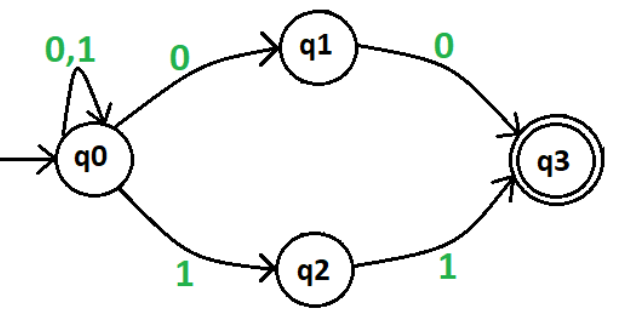
\includegraphics[scale = 0.3]{media/diagramma_stato.png}
\centering
\caption{Diagramma di transizione}
\end{figure}

\subsubsection*{ Tabelle di transizione }
Una tabella di transizione è costituita nelle riga dalle funzioni $\delta$ e nelle colonne dagli input. Ogni incrocio equivale a uno stato della funzione $\delta$ con un input generico \emph{a}.

\begin{table}[h]
\centering
\begin{tabular}{c | c | c}
& 0 & 1 \\
\hline
$\rightarrow$  q\textsubscript{0} & q\textsubscript{2} & q\textsubscript{0} \\
$*$q\textsubscript{1} & q\textsubscript{1} & q\textsubscript{1} \\
q\textsubscript{2} & q\textsubscript{2} & q\textsubscript{1} \\
\end{tabular}
\caption{Esempio di tabella}
\end{table}

La freccia è lo start e l'asterisco è lo stato finale.

\subsubsection{ Estensione della funzione di transizione di stringhe }
Allo scopo di poter seguire una sequenza di input ci serve definire una funzione di transizione estesa. Se $\delta$ è una funzione di transizione, chiameremo \circumdelta\space la sua funzione estesa.
La funzione estesa prende in input \emph{q} e una stringa \emph{w} e ritorna uno stato \emph{p}. 
\\ Ogni stato viene calcolato grazie allo stato esteso precedente: \[\circumdelta(\emph{q,w}) = \delta(\circumdelta(\emph{q,x}), \emph{a})\]
\subsubsection*{Esempio}
L = \{ \emph{w} $|$ \emph{w} ha un numero pari di 0 e di 1 \}
\\ Nota bene: 0 (numero di simboli) è pari quindi conta come stato accettato, ed è l'unico stato accettato. 
\\ \hspace*{0.4cm} q\textsubscript{0}: 0 e 1 sono pari
\\ \hspace*{0.4cm} q\textsubscript{1}: 0 pari 1 dispari
\\ \hspace*{0.4cm} q\textsubscript{2}: 1 pari 0 dispari
\\ \hspace*{0.4cm} q\textsubscript{3}: 0 dispari 1 dispari
\[A = (\{q0,q1,q2,q3\}, \{0,1\}, \delta, q\textsubscript{0}, \{q\textsubscript{0}\})\]

\begin{figure}[h]
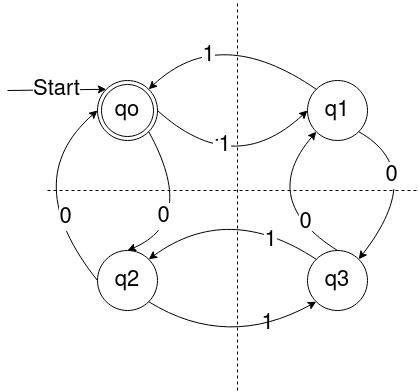
\includegraphics[scale = 0.5]{media/stringhe_pari.png}
\centering
\caption{Diagramma}
\end{figure}

\begin{table}[ht]
\centering
\begin{tabular}{c | c | c}
& 0 & 1 \\
\hline
$\rightarrow *$ q\textsubscript{0} & q\textsubscript{2} & q\textsubscript{1} \\
q\textsubscript{1} & q\textsubscript{3} & q\textsubscript{0} \\
q\textsubscript{2} & q\textsubscript{0} & q\textsubscript{3} \\
q\textsubscript{3} & q\textsubscript{1} & q\textsubscript{2} \\
\end{tabular}
\caption{Esempio funzioni}
\end{table}

\newpage
Ora applichiamo le funzione di transizione estesa per verificare che 110101 abbia 0 e 1 pari: 
\begin{itemize}
\item  \circumdelta$(q\textsubscript{0}, \epsilon)$ = q\textsubscript{0}
\item  \circumdelta$(q\textsubscript{0}, 1)$ = $\delta(\circumdelta(q\textsubscript{0}, \epsilon),1)$ = $\delta(q\textsubscript{0},1)$ =  q\textsubscript{1}
\item  \circumdelta$(q\textsubscript{0}, 11)$ = $\delta(\circumdelta(q\textsubscript{0}, 1),1)$ = $\delta(q\textsubscript{1},1)$ =  q\textsubscript{0}
\item  \circumdelta$(q\textsubscript{0}, 110)$ = $\delta(\circumdelta(q\textsubscript{1}, 11),0)$ = $\delta(q\textsubscript{0},1)$ =  q\textsubscript{2}
\item  \circumdelta$(q\textsubscript{0}, 1101)$ = $\delta(\circumdelta(q\textsubscript{0}, 110),1)$ = $\delta(q\textsubscript{2},1)$ =  q\textsubscript{3}
\item  \circumdelta$(q\textsubscript{0}, 11010)$ = $\delta(\circumdelta(q\textsubscript{0}, 1101),0)$ = $\delta(q\textsubscript{3},0)$ =  q\textsubscript{1}
\item  \circumdelta$(q\textsubscript{0}, 110101)$ = $\delta(\circumdelta(q\textsubscript{0}, 11010),1)$ = $\delta(q\textsubscript{1},1)$ =  q\textsubscript{0}

\end{itemize}
A ogni simbolo aggiunto posso usare la funzione estesa precedente per calcolare il prossimo stato, in questo caso la sequenza ha un numero pari di 0 e 1.

\section{Automa a stati finiti non deterministici}
Un NFA (nondeterministic finite automaton) può trovarsi contemporaneamente in diversi stati. L'automa "scommette" sul input su certe proprietà dell'input.
\\ I NFA sono spesso più succinti e facili da definire rispetto ai DFA, un DFA può avere un numero di stati addirittura esponenziale rispetto a un NFA. Ogni NFA può essere convertito in un DFA.

\newpage
\subsection{Descrizione informale}
A differenza di un DFA, una funzione di stato in un NFA può restituire 0 o più stati. Immaginiamo di dover identificare se una stringa finisce con 01. 
\\ Di seguito il diagramma di transizione sarà il seguente.
\begin{figure}[h]
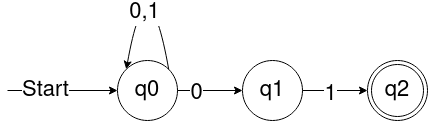
\includegraphics[scale = 0.5]{media/01_end.png}
\centering
\caption{NFA che accetta stringa che finisce con 01}
\end{figure}
Come è possibile notare q\textsubscript{0} può può restituire due stati se riceve uno 0. Il NFA esegue molteplici stadi alla ricerca del pattern (simile a un processo che si moltiplica). 

\begin{figure}[h]
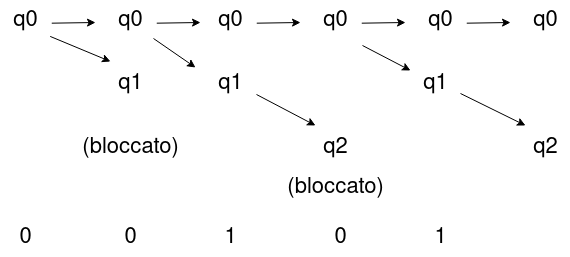
\includegraphics[scale = 0.5]{media/NFA_es.png}
\centering
\caption{Gli stati del NFA}
\end{figure}
Ogni volta che il NFA accetta uno stato 0 crea due processi, un q\textsubscript{1} e q\textsubscript{0}
A ogni successivo input tutti i processi vanno avanti, nel nostro caso il q\textsubscript{1} "muore". Al secondo giro viene creato q\textsubscript{1} che muore alla quarta iterazione perché non è l'ultimo simbolo. Durante la quarta iterazione nasce q\textsubscript{1} che alla quinta ci porta uno stato accettato.

\newpage
\subsection{Definizione formale}
Formalmente un NFA si definisce come un DFA.
\[A = (Q, \Sigma, \delta, q\textsubscript{0}, F)\]
\begin{enumerate}
  \item Un insieme di stati finiti Q
  \item Un insieme di simboli di input, $\Sigma$
  \item Una funzione di transizione, che prende in input uno stato e un simbolo e restituisce \emph{\textbf{un insieme di stati}}. Questa è l'unica differenza rispetto al DFA, dove ci viene restituito un singolo stato.
  \item Uno stato iniziale (naturalmente che appartiene a Q)
  \item Un insieme di stati accettati finali F. Questo è un sottoinsieme di Q.
\end{enumerate}

\begin{table}[ht]
\centering
\begin{tabular}{c || c | c}
& 0 & 1 \\
\hline\hline
  $\rightarrow$ q\textsubscript{0} & \{q\textsubscript{0}, q\textsubscript{1}\} & \{q\textsubscript{0}\} \\
q\textsubscript{1} & $\emptyset$ & \{q\textsubscript{2}\} \\
$*$q\textsubscript{2} & $\emptyset$ & $\emptyset$ \\
\end{tabular}
\caption{Tabella di transizione di una NFA che accetta una stringa che finisce con 01}
\end{table}
L'unica differenza con una tabella DFA è che negli incroci ci sono dei insiemi di stati di output (singoletto quanto è uno solo), mentre se la transizione non esiste viene segnata con $\emptyset$.

\newpage
\subsection{Funzione di transizione estesa}
Come per i DFA bisogna prendere la funzione di transizione e renderla estesa. In questo caso lo stato precedente può ritorna un insieme di stati, quindi bisognare fare l'unione di questi. La funzione estesa di $\delta$ si chiamerà \circumdelta. 
\[\bigcup^k_{x=2}\delta(p_i,a) = \{r_1,r_2,... ,r_m\} \]
Usiamo \circumdelta\space per calcolare se la stringa 00101 finisce con 01. 

\begin{enumerate}
  \item $\circumdelta(q_0, \epsilon) = \{q_0\}$
  \item $\circumdelta(q_0, 0) = \delta(q_0,0) = \{q_0, q_1\}$
  \item $\circumdelta(q_0, 00) = \delta(q_0,0) \cup \delta(q_1,0)  = \{q_0, q_1\} \cup \emptyset = \{q_0, q_1\} $
  \item $\circumdelta(q_0, 001) = \delta(q_0,1) \cup \delta(q_1, 1) = \{q_0\} \cup \{q_2\} = \{q_0, q_2\}$
  \item $\circumdelta(q_0, 0010) = \delta(q_0,0) \cup \delta(q_2, 0) = \{q_0, q_1\} \cup \emptyset = \{q_0, q_1\}$
  \item $\circumdelta(q_0, 00101) = \delta(q_0,1) \cup \delta(q_1, 1) = \{q_0\} \cup \{q_2\} = \{q_0, q_2\}$
\end{enumerate}
Abbiamo un risultato positivo, $q_2$ mentre $q_0$ viene scartato

\subsection{Linguaggio NFA} 
Come abbiamo visto sopra, il fatto di avere uno stato non accettabile al termine dell'operazione non significa che non abbia avuto successo. 
\\ Formalmente se $A = (Q, \Sigma, \delta, q\textsubscript{0}, F)$ è un NFA allora: 
\[L(A) = \{ w | \circumdelta(q_0, w) \cap \emph{F} \ne \emptyset \}\]
In parole povere L(A) è l'insieme delle stringhe w in $\Sigma^*$ tale che \circumdelta($q_0,w)$ contenga almeno uno stato accettante.

\newpage
\subsection{Equivalenza tra DFA e NFA}
Di solito è più facile ottenere un NFA piuttosto che un DFA per un linguaggio. Nel migliori dei casi un DFA ha circa tanti stati quanti un NFA, ma più transizioni. Nel caso peggiore un DFA ha $2^n$ stati, mentre un NFA n.
\\ Come detto in precedenza ogni NFA può essere ricondotto a un DFA, questo andrà dimostrato costruendo un DFA per insiemi a partire da un NFA. 
\\ Dato un NFA $A = (Q_N, \Sigma, \delta_N, q\textsubscript{0}, F_N)$ possiamo costruire un DFA \\ $A = (Q_D, \Sigma, \delta_D, \{q_0\}, F_D)$ tale che L(D)=L(N) (che i linguaggio sono uguali).
\\ Si noti che i due linguaggi condividono lo stesso alfabeto.
\\ Gli altri D componenti sono fatti nel seguente modo: 
\begin{outline}
  \1 $Q_D$ è formato da un insieme di insiemi di $Q_N$, in termini formali $Q_D$ è l'insieme potenza di $Q_N$. Quindi se $Q_N$ ha \emph{n} stati allora $Q_D$ ha $2^n$ stati, questo è vero nella teoria, nella pratica gli stati non raggiungibili non contano quindi tendono a essere meno di $2^n$.
  \1 $F_D$ è l'insieme dei sottoinsiemi di S di $Q_N$ tale che \emph{S}$ \cap F_N \ne \emptyset$. $F_D$ è quindi formato dagli sottoinsiemi di stati \emph{N} che includono almeno uno stato accettante.
  \1 Per ogni insieme \emph{S} $\subseteq Q_N$ e per ogni simbolo \emph{a} in $\Sigma$, 
  \[\delta_D(S,a) = \bigcup_{p\;in\;S} \delta_N(p,a)\]
\end{outline}
  Ovvero l'insieme $\delta_D(S,a)$ è calcolato tramite l'unione di tutti gli insiemi p in S.
\begin{table}[ht]
\centering
\begin{tabular}{c || c | c}
& 0 & 1 \\
\hline \hline
  $ \emptyset $ & $ \emptyset $ & $ \emptyset $ \\
  $ \rightarrow \{q_0\} $ & $ \{q_0, q_1\} $ & $ \{q_0\} $ \\
  $ \{q_1\} $ & $ \emptyset $ & $ \{q_2\} $ \\
  $ *\{q_2\} $ & $ \emptyset $ & $ \emptyset $ \\
  $ \{q_0,q_1\} $ & $  \{q_0, q_1\} $ & $ \{q_0,q_2\} $ \\
  $ *\{q_0,q_2\} $ & $ \{q_0, q_1\} $ & $ \{q_0\} $ \\
  $ *\{q_1,q_2\} $ & $ \emptyset $ & $ \{q_2\} $ \\
  $ *\{q_0, q_1, q_2\} $ & $ \{q_0,q_1\} $ & $ \{q_0,q_2\} $ \\
\end{tabular}
\caption{Stringa che termina con 01, NFA $\rightarrow$ DFA}
\end{table}

La tabella precedente era deterministica nonostante fosse formata da insiemi, \emph{ogni insieme è uno stato}, e non sono insieme di stati. Per rendere più chiara l'idea possiamo cambiare notazione.
\begin{table}[ht]
\centering
\begin{tabular}{c || c | c}
& 0 & 1 \\
\hline \hline
  \hphantom{*$\rightarrow$}A& A & A \\
  \hphantom{*}$\rightarrow$B & E & B \\
  \hphantom{*$\rightarrow$}C & A & D \\
  \hphantom{$\rightarrow$}$*$D & A & A \\
  \hphantom{*$\rightarrow$}E & E & F \\
  \hphantom{$\rightarrow$}$*$F & E & B \\
  \hphantom{$\rightarrow$}$*$G & A & D \\
  \hphantom{$\rightarrow$}$*$H & E & F \\
\end{tabular}
\caption{Stringa che termina con 01, notazione nuova}
\end{table}
\\ Tra gli 8 stati presenti in tabella possiamo raggiungere: B, E e F. Gli atri stati sono irraggiungibili o non esistenti. È possibile evitare di costruire questi stati compiendo una "valuta differita".
\\ Trattando i l'insieme di stati come un unico stato composto da un insieme è possibile riscrivere la DFA in questo modo: 

\begin{figure}[h]
  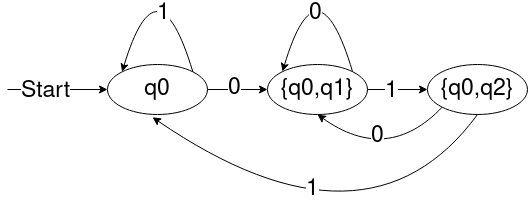
\includegraphics[scale = 0.5]{media/nfa_to_dfa.png}
\centering
\caption{Grafico DFA convertito da NFA}
\end{figure}

\newpage
\subsection*{} 
\subsubsection*{Teorema}
Se $D = (Q_N, \Sigma, \delta_N, q\textsubscript{0}, F_N)$ è il DFA trovato per costruzione a partire dal NFA $N = (Q_D, \Sigma, \delta_D, \{q_0\}, F_D)$ allora L(D)=L(N).

\subsubsection*{Teorema}
Un linguaggio L è accettato da un DFA se e solo se L è accettato da un NFA.

\newpage
\section{Automa con epsilon-transazioni}
Un estensione degli automa è la capacita di poter ammettere come input la stringa vuota $\epsilon$. È come se l'NFA compisse una transizioni spontaneamente. Tale NFA si chiamerà $\epsilon$-NFA

\subsection{Uso delle epsilon-transizioni}
L'esempio di seguito tratta le $\epsilon$ come invisibili, possono mutare lo stato ma non sono contante nella catena. 

\begin{figure}[h]
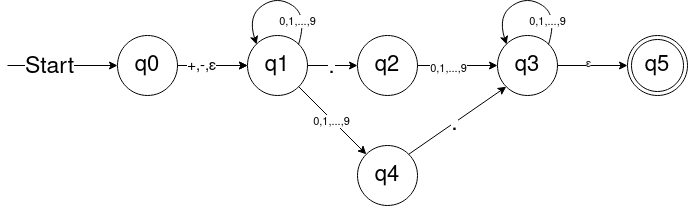
\includegraphics[scale = 0.5]{media/epsilon_nfa.png}
\centering
\caption{epsilon-NFA che accetta numeri decimali}
\end{figure}

L'$\epsilon$-NFA in figura accetta numeri decimali formati da: 
\begin{enumerate}
  \item un segno +,- facoltativo
  \item una sequenza di cifre
  \item un punto decimale
  \item una seconda sequenza di cifre
\end{enumerate}
È possibile avere input vuoti prima della virgola $\delta(q_1, .) = q_2$ e dopo la virgola $\delta(q_4, .) = q_3$ ma non entrambi. Il segno è facoltativo $\delta(q_0, \epsilon) = q_1$.
\\ In $q_3$ l'automa può "scommettere" che la sequenza sia finita oppure può andare avanti a leggere.

\newpage
\subsection{Notazione formale di epsilon-NFA}
La definizione forma di un $\epsilon$-NFA è uguale a quella di un NFA, va solo specificate le informazioni relative alla transizione $\epsilon$.
\\ Una $\epsilon$-NFA è definita con $A = (Q, \Sigma, \delta, q_0, F)$, dove $\delta$ è una funzione di transizione che richiede come input: 
\begin{enumerate}
  \item uno stato \emph{Q}
  \item un elemento $\Sigma \cup \{\epsilon\}$, ovvero un simbolo di input oppure il simbolo $\epsilon$. Questa distinzione viene fatta per evitare confusione. 
\end{enumerate}

$\epsilon$-NFA per riconoscere un numero decimale
\[ E = (\{q_0,q_1,...,q_5\}, \{.,+,-,1,...,9\},\delta, q_0, \{q_5\})\]

\begin{table}[ht]
\centering
\begin{tabular}{c || c | c | c | c}
& $\epsilon$ & +,- & . & 0,1,...,9 \\
\hline \hline
  $q_0$ & $\{q_1\}$ & $\{q_1\}$ & $\emptyset$ & $\emptyset$ \\
$q_1$ & $\emptyset$ & $\emptyset$ & $\{q_2\}$ & $\{q_1, q_4\}$ \\
$q_2$ & $\emptyset$ & $\emptyset$ & $\emptyset$ & $\{q_3\}$ \\
$q_3$ & $\{q_5\}$ & $\emptyset$ & $\emptyset$ & $\{q_3\}$ \\
$q_4$ & $\emptyset$ & $\emptyset$ & $\{q_3\}$ & $\emptyset$ \\
$q_5$ & $\emptyset$ & $\emptyset$ & $\emptyset$ & $\emptyset$ \\
\end{tabular}
\caption{Tabella di transizione per un numero decimale}
\end{table}

\subsection{Epsilon chiusure}
Un $\epsilon$-chiusura è un cammino fatto solo di transizioni $\epsilon$. Formalmente tale stato si scrive ENCLOSE(q) = {insieme di stati.}

\subsection{Transizioni estese di epsilon-NFA}
Grazie alle $\epsilon$-chiusure possiamo definire cosa significa accettare un input.






\section{Esercitazioni} 
\subsection{Esercitazione 09/21/23}
\subsubsection{Costruzione DFA}
Consideriamo l'alfabeto \{a,b\}. 
Realizzare dei DFA che riconoscono i seguenti linguaggi:
\begin{enumerate}
  \item stringhe con un numero dispari di a 
\\ SI ab,aaa,bba,aaba
\\ NO $\epsilon$,aa

\begin{figure}[h]
  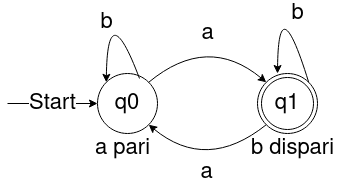
\includegraphics[scale = 0.5]{media/09_21_es1.png}
  \centering
\end{figure}

\item 
stringhe che terminano con bb
\\ SI bb,babb
\\ NO $\epsilon$,ba,a,aba

\begin{figure}[h]
  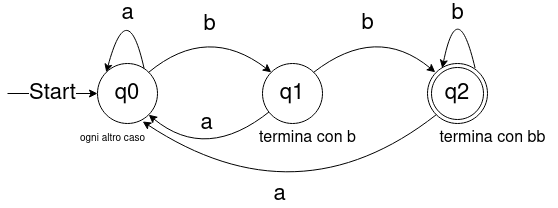
\includegraphics[scale = 0.5]{media/09_21_es2.png}
  \centering
\end{figure}

\newpage
\item stringhe che non terminano con bb
\\ SI $\epsilon$,ba,a,aba
\\ NO bb,babb

\begin{figure}[h]
  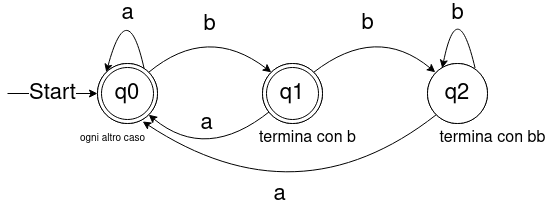
\includegraphics[scale = 0.5]{media/09_21_es3.png}
  \centering
\end{figure}

\newpage
\item stringhe con un numero pari di a ed almeno 3 b
\\ SI bbb,bababb
\\ NO $\epsilon$,bbaa,bababa

\begin{figure}[h]
  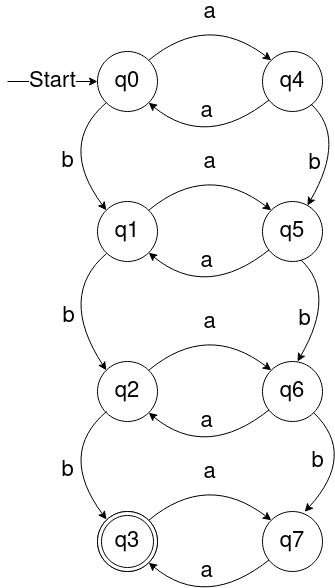
\includegraphics[scale = 0.5]{media/09_21_es4.png}
  \centering
\end{figure}

\newpage
\item stringhe che contengono la sottostringa aaa o la sottostringa aba (contengono almeno una delle due)
\\ SI babab,aaaa,aaaba
\\ NO $\epsilon$,abba,a,b,ab

\begin{figure}[h]
  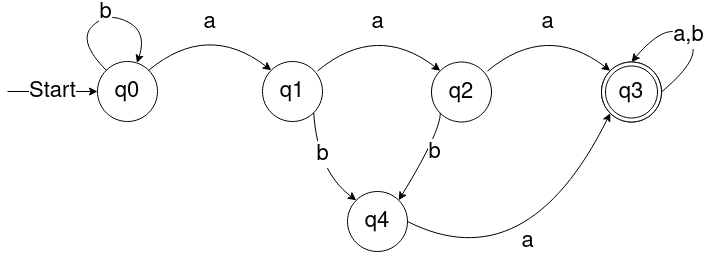
\includegraphics[scale = 0.5]{media/09_21_es5.png}
  \centering
\end{figure}

\item Realizzare un DFA che riconosca il seguente linguaggio su alfabeto \{0,1\}: stringhe che interpretate come numero binario risultano un multiplo di 5 
\\
SI 101,1010,1111,0
\\
NO 111,1,10

\begin{figure}[h]
  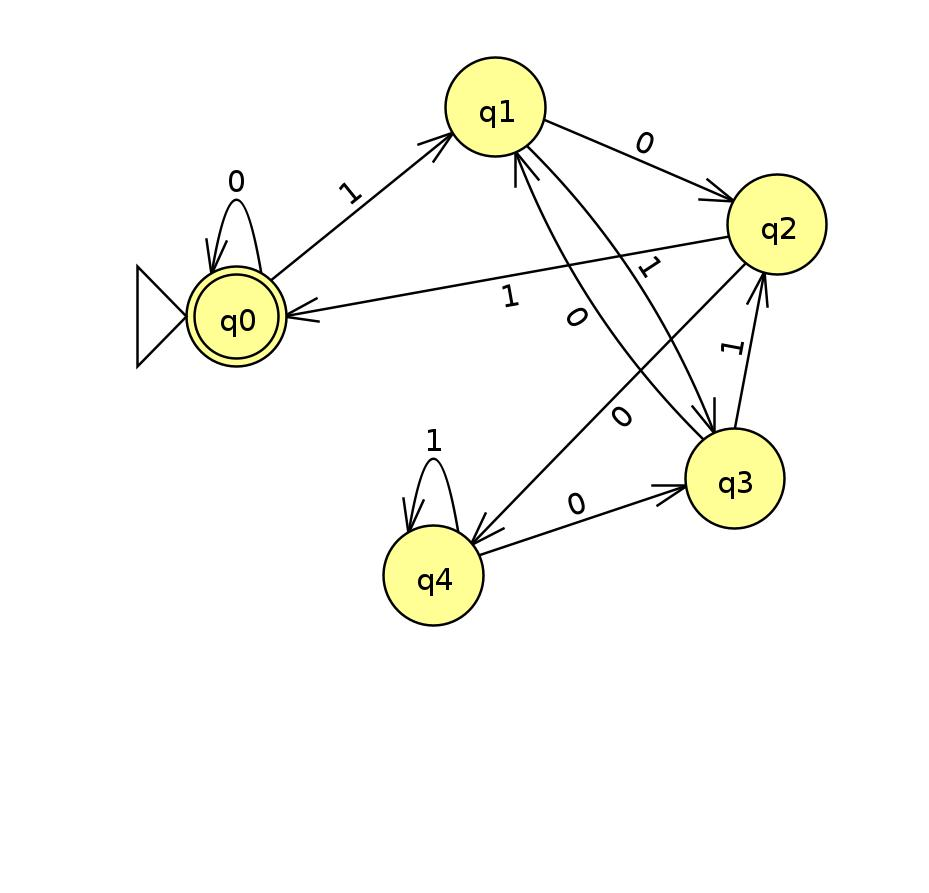
\includegraphics[scale = 0.25]{media/09_21_es6.jpg}
  \centering
\end{figure}
NB: Devi considerare tutti i numeri fino a 5!

\item Sempre considerando alfabeto \{0,1\}, realizzare un DFA che controlla la correttezza delle somme binarie: data la stringa: $a_0 b_0 c_0 a_1 b_1 c_1 ... a_n b_n c_n$ controlla se $a_n...a_1 a_0 + b_n...b_1 b_0 = c_n...c_1 c_0$ (cioè a+b=c con a,b,c numeri binari con stessa lunghezza) 

\begin{figure}[h]
  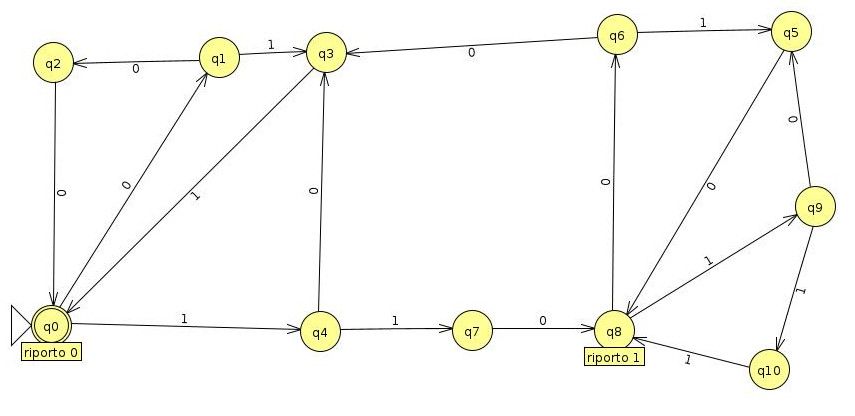
\includegraphics[scale = 0.4]{media/09_21_es7.jpg}
  \centering
\end{figure}

Non mi torna...

\end{enumerate}

\newpage
\subsubsection{NFA}
\begin{enumerate}
  \item 
    Dato l'alfabeto \{a,b\} realizzare un NFA che riconosce le stringhe che 
    contengono aaa oppure aba
    \\
    SI babab,aaaa,aaaba
    \\
    NO $\epsilon$,abba,a,b,ab

\begin{figure}[h]
  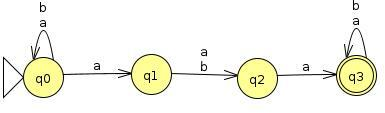
\includegraphics[scale = 0.5]{media/es8.jpg}
  \centering
\end{figure}

  \item Realizzare un NFA che riconosce le stringhe non vuote sull'alfabeto \{0,1,2\} in cui l'ultima cifra appare almeno una volta in precedenza
    \\
    SI 011,121,22,0120
    \\
    NO $\epsilon$,012,20,1

\begin{figure}[h]
  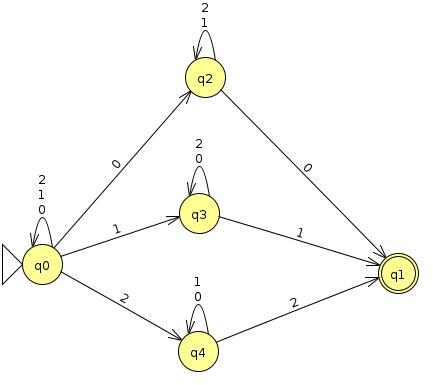
\includegraphics[scale = 0.5]{media/es9.jpg}
  \centering
\end{figure}

\newpage
\item Realizzare un NFA che riconosce le stringhe non vuote sull'alfabeto {0,1,2} in cui l'ultima cifra NON appare in precedenza
\\
SI 012,20,1
\\
NO $\epsilon$,011,121,22,0120

\begin{figure}[h]
  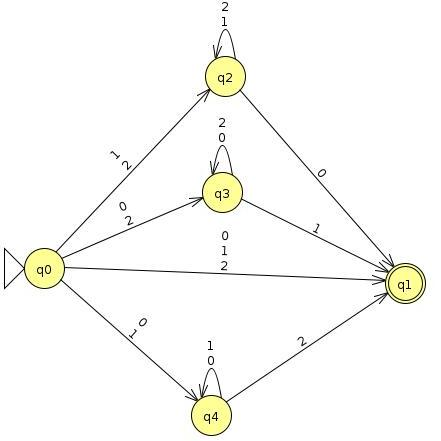
\includegraphics[scale = 0.5]{media/es10.jpg}
  \centering
\end{figure}

\end{enumerate}
\end{document}
